%\documentclass{article}
%\usepackage{graphicx,subfigure}
%\begin{document}

\begin{figure}[!h]
  \centering
  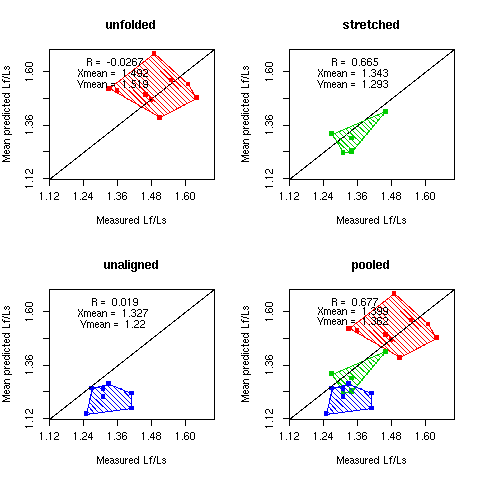
\includegraphics[width=1.1\textwidth]{figfcpredlfr.png}
% original is nfc.5.10.predlfr.png
  \caption{Plots of measured fibre length to staple length ratio against predicted mean fibre length to staple length ratio with predictions based on measurement of wavelength and amplitude by the FC technique. Fibre lengths for the unfolded crimp type wools were adjusted for the effect of twist at the points of inflection using $H = 0.5 * amplitude$ and $R = 0.10 mm$ in the prediction equations.}
  \label{fig:fcpredlfr}
\end{figure}

%\end{document}

